\chapter{Consensus}
\section{Motivation}
Many algorithms require a set of processes running in a distributed system to agree on values (e.g order of messages, program state).
\begin{itemize}
    \item Processes each propose a value, some agreement algorithm occurs, and then all decide on the same value.
    \item Required for all processes to get a consistent view, even if a single leader decided on a value there would then be a consensus required on which process is the leader to start, and when leaders fail.
    \item Often a \textit{replicated server/replica} stores the state replicated over all processes (e.g the sequence of transactions for a database, the current player count in a game).
\end{itemize}

\begin{definitionbox}{Uniform Consensus}
    \begin{center}
        \begin{tabular}{l l p{.6\textwidth}}
            \textbf{Validity} & Safety & If a process decides on a value, then this value was proposed by some process. \\
            \textbf{Integrity} & Safety & A process can only decide on one value at most. \\
            \textbf{Termination} & Liveness & Each correct process eventually decides. \\
            \textbf{Uniform Agreement} & Safety & Processes cannot decide on different values. \\
        \end{tabular}
    \end{center}
\end{definitionbox}

\begin{definitionbox}{Regular Consensus}
    A strengthening of \textit{Uniform Consensus} to replace \textbf{Uniform Agreement}.
    \begin{center}
        \begin{tabular}{l l p{.6\textwidth}}
            \multicolumn{3}{c}{\textbf{Validity, Integirty and Termination Properties from Uniform Consensus}} \\
            \textbf{Uniform Agreement} & Safety & \textbf{Correct} Processes cannot decide on different values. \\
        \end{tabular}
    \end{center}
\end{definitionbox}

\section{Primary Backup}
A simple consensus algorithm between two servers.
\begin{center}
    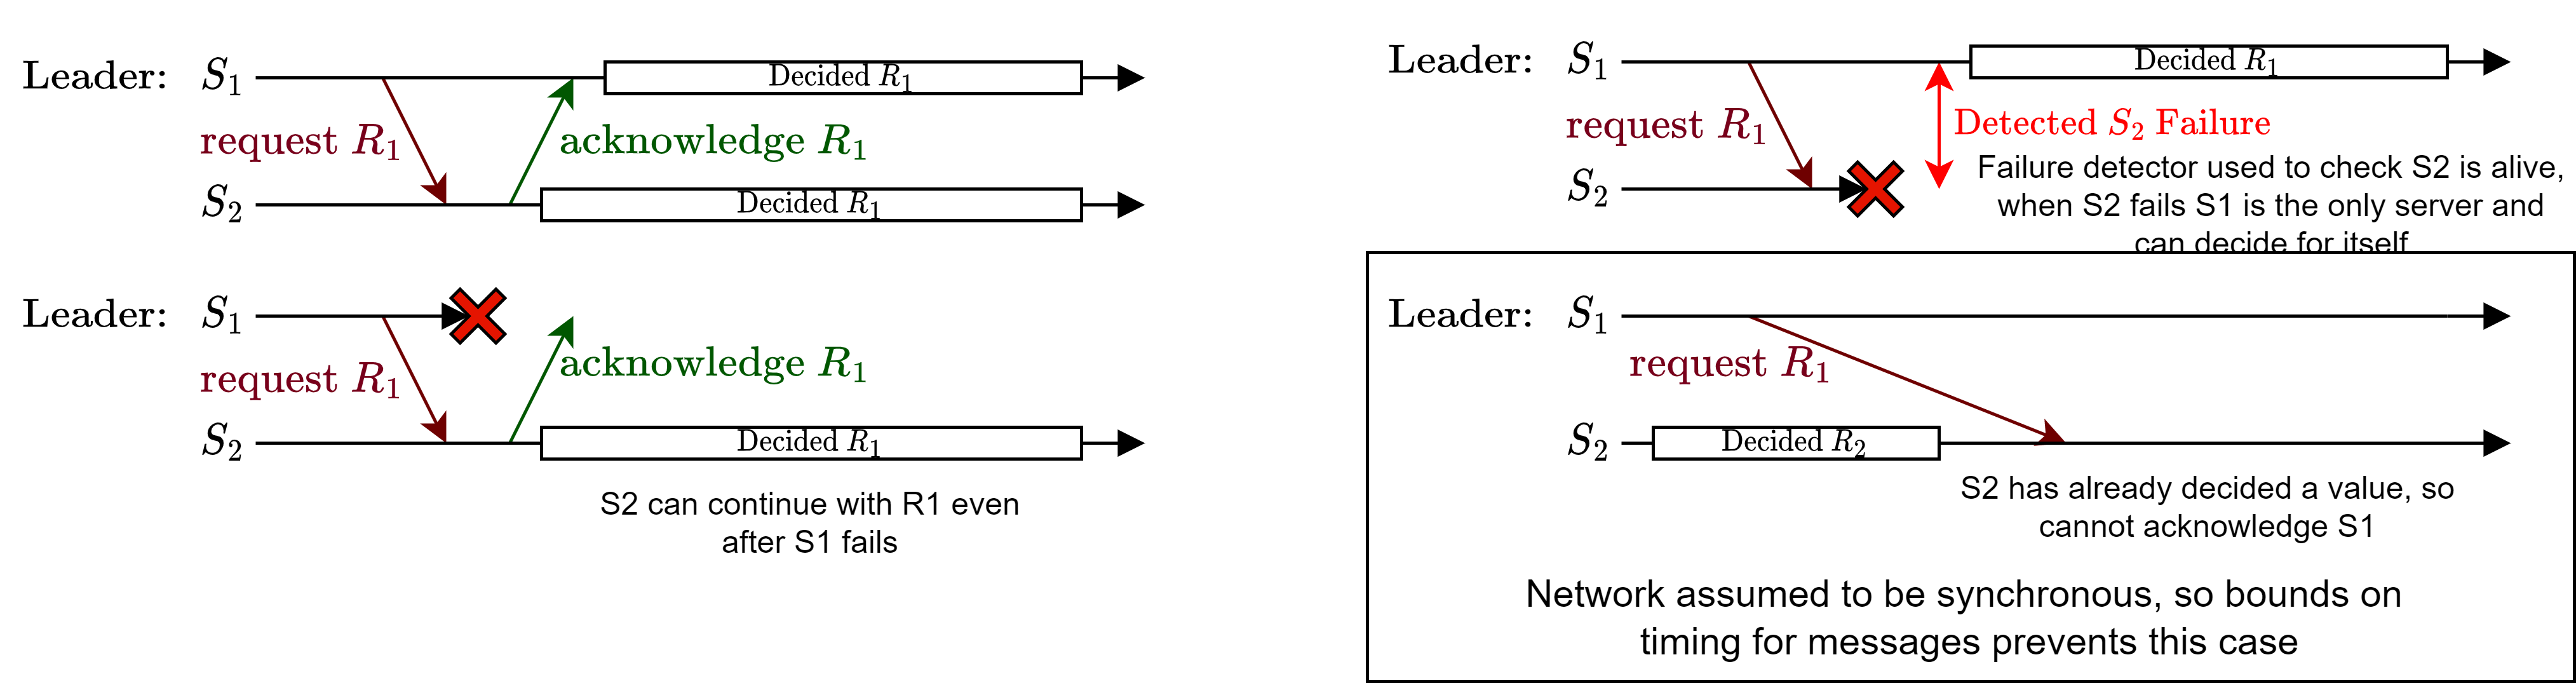
\includegraphics[width=.9\textwidth]{consensus/images/primary_backup_scenarios.drawio.png}
\end{center}
\begin{itemize}
    \item One server is the leader, a failure detector is used by the leader to check the other server.
    \item Only works in a synchronous system (time bound on all messages), violations on order of requests, and timing will violate consensus.
\end{itemize}

\section{FLP Impossibility Result}
% FLP Impossibility Result Lecture
% In a purely asynchronous system we cannot use message timings to determine if a process has crashed (no guarentee on timings)
% 
% Applies even when:
% Single bit
% Reliable message passing
% Only one process crashes
%
% Can be side stepped with synchronous systems or unreliable failure detectors
% 
\unfinished



\section{Common Consensus Algorithms}
\begin{center}
    \begin{tabular}{l p{.7\textwidth}}
        \textbf{Multipaxos} & Most popular algorithm, variants are used across industry; Google chubby (a distributed lock manager), BigTable (a Google DBMS), AWS, Azure Fabric, Neo4j (a graph DBMS), Apache Mesos (a distributed systems kernel). \\
        \textbf{Raft} & (\textbf{R}eliable, \textbf{R}eplicated, \textbf{R}edundant \textbf{A}nd \textbf{F}ault \textbf{T}olerant)A newer algorithm (formally verified, and easier to understand) used in Meta's \href{https://engineering.fb.com/2014/06/05/core-data/hydrabase-the-evolution-of-hbase-facebook/?__xts__%5B0%5D=68.ARAXKR3kWX0_4Qq8xe7s2lwVPwGcEZrV8OV-K16hi-eK-Fb1LzlWDazInohFF1g7XTiHMwRkIQAtaF4yR04WO2-OChkq5L-JZZHw910Bm5FOlY0ZFRxo4Y65ZK6ovA3CUbcKPshN0nWFN6Z62CkA-27w-3fVqnQFkSajsljxYeg55G3wHfhbDBRBWNeOAoyTy2lLuocoxiWziROo5yQVrWJxMBH-f2cLHvJmXgcAqirctOmnxjsHDa5zzeJLHaxQVLv7KCCo3B3-8QTPNh-LhwrU34PvQEr5-0KajxXw4ruOLunEMQ&__tn__=HHH-R}{Hydrabase}, Kubernetes and Docker Swarm. \\ 
        \textbf{PBFT} & (\textbf{P}ractical \textbf{B}yzantine \textbf{F}ault \textbf{T}olerance) and proof of work/proof of stake are used for many blockchains backing cryptocurrencies such as Bitcoin. \\
        \textbf{Viewstamped Replication} & An early consensus algorithm designed to be easily added to non-distributed programs, it has been improved upon with \href{https://pmg.csail.mit.edu/papers/vr-revisited.pdf}{VSR Revisited}. \\
        \textbf{Atomic Broadcast} & Implemented in Apache Zookeeper (ZAB protocol) for building coordination services and is used for services such as Apache Hadoop (similar to MapReduce). \\
        \textbf{CRDTs} & (\textbf{C}onflict-\textbf{F}ree \textbf{R}eplicated \textbf{D}atatypes) A data structure that can be updated independently \& across a distributed system and can resolve any inconsistencies itself, with all eventually converging to the same value. \\
    \end{tabular}
\end{center}

\section{Paxos}
\begin{definitionbox}{Paxos}
    A consensus algorithm wherein each server has:
    \begin{center}
        \begin{tabular}{l p{.8\textwidth}}
            \textbf{Learner} & Receives decisions, alters the state based on agreed values. \\
            \textbf{Proposer} & Proposes values to \textbf{Acceptor}s, associated with its proposal number. Receives accepted values. \\
            \textbf{Acceptor} & Accepts values with increasing ballot numbers. \\
        \end{tabular}
    \end{center}
\end{definitionbox}
\begin{center}
    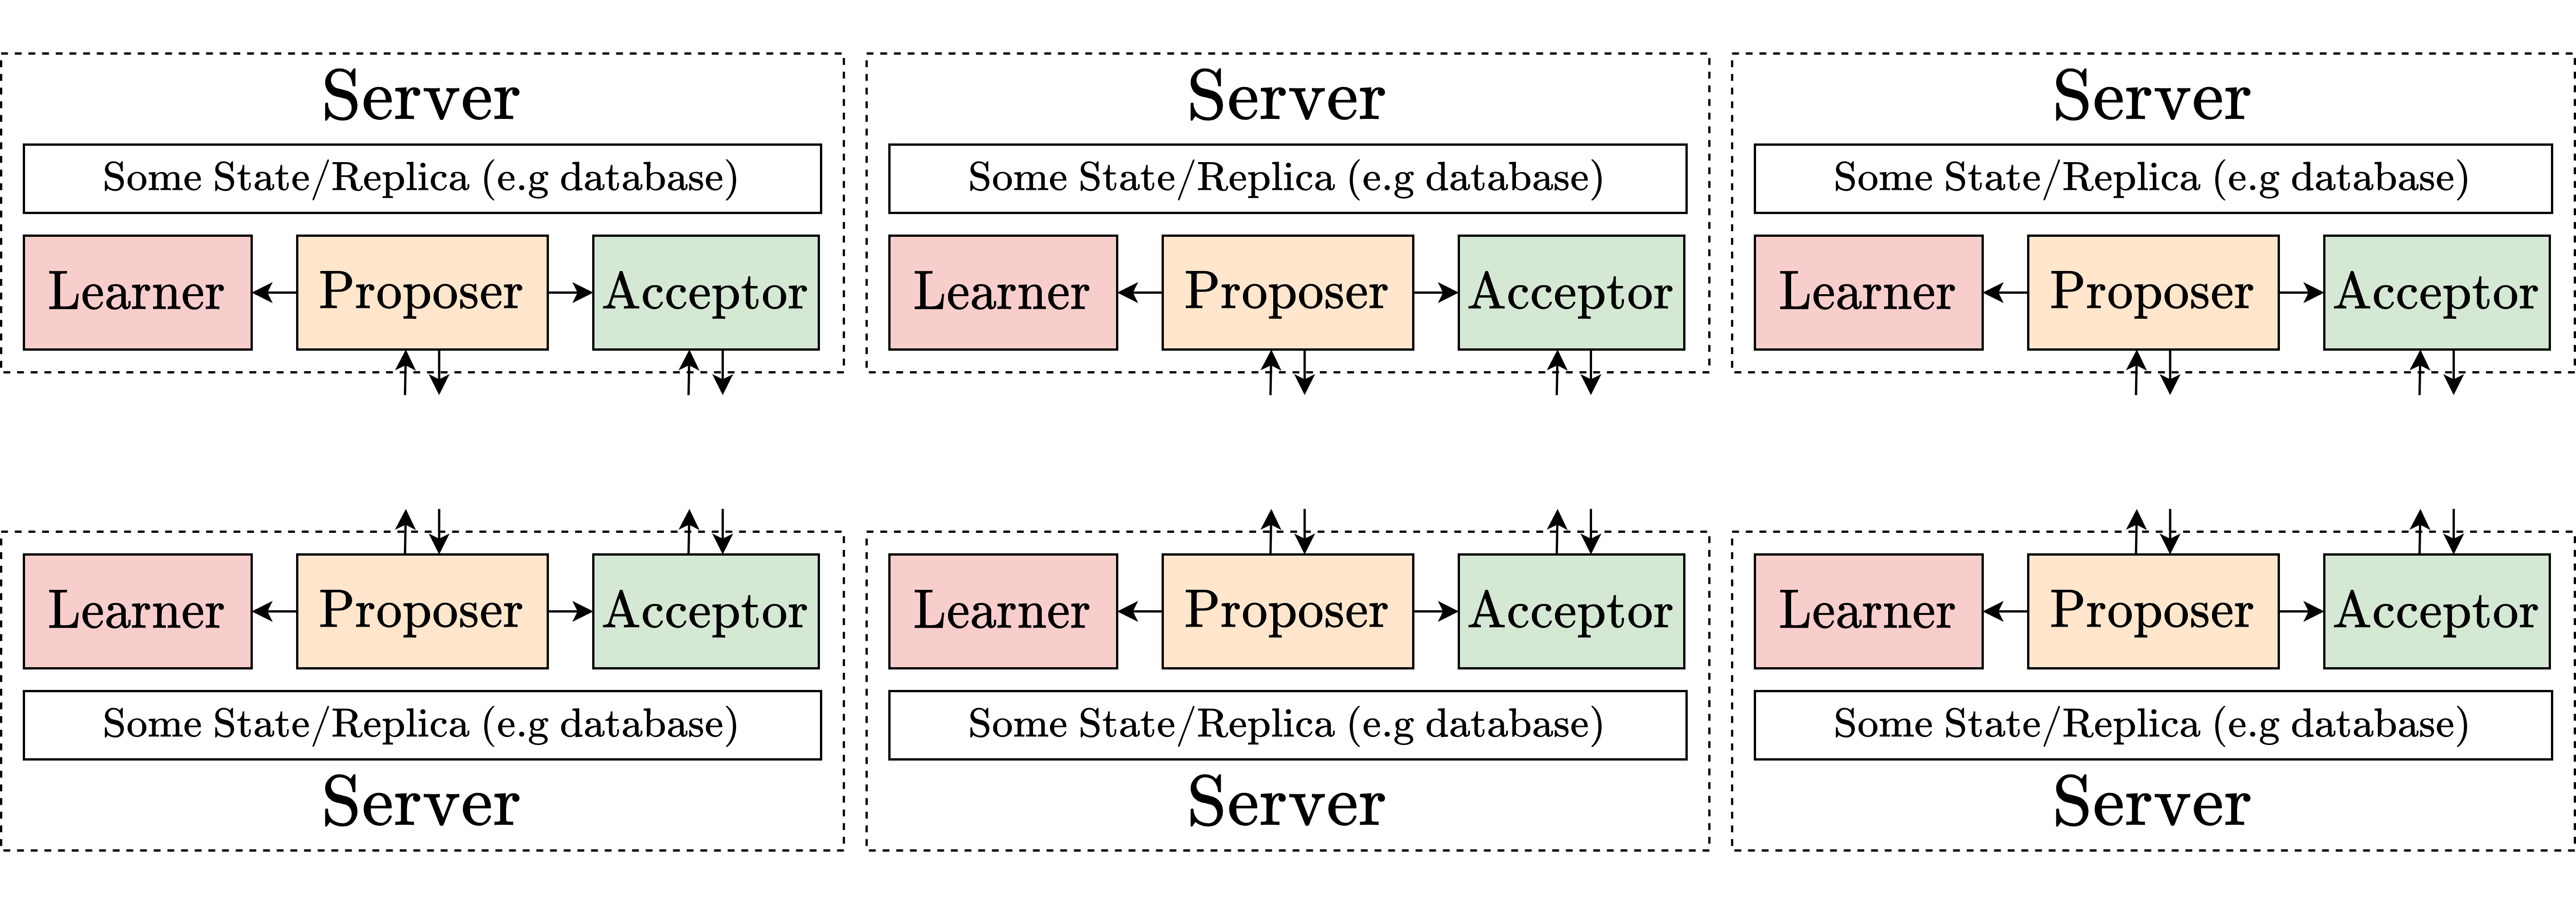
\includegraphics[width=\textwidth]{consensus/images/paxos_servers.drawio.png}
\end{center}

\begin{center}
    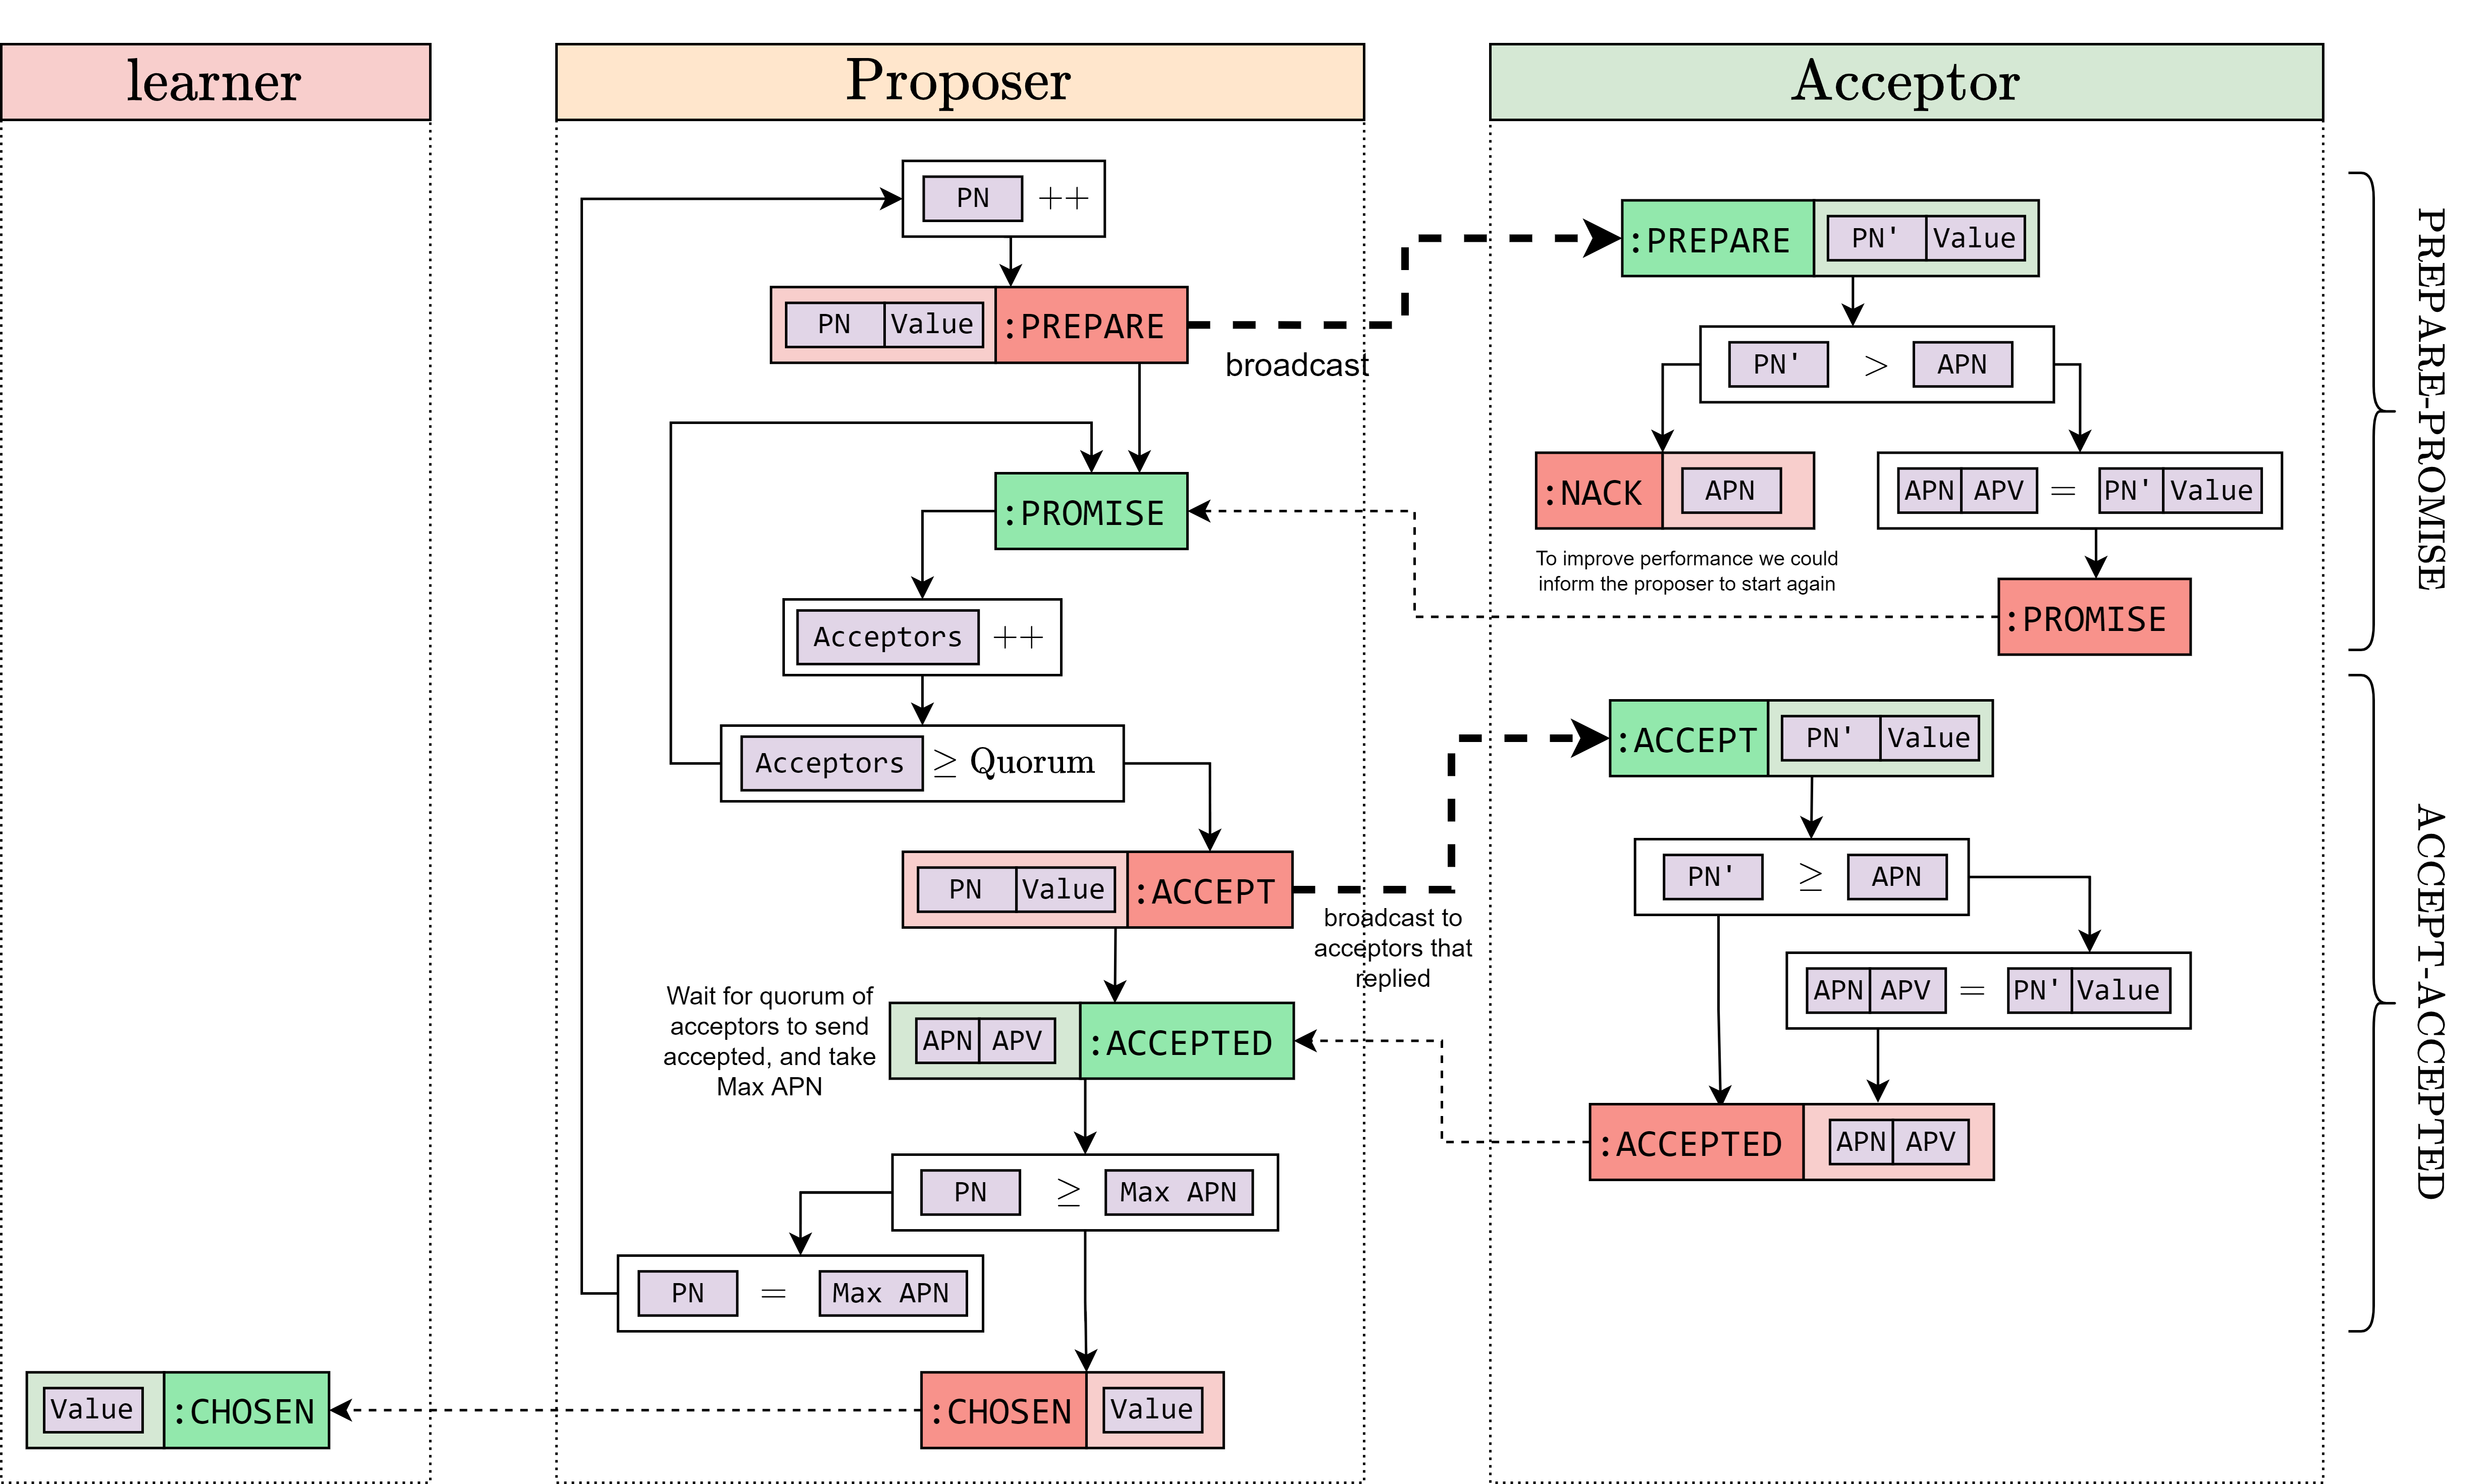
\includegraphics[width=\textwidth]{consensus/images/paxos_stages.drawio.png}
\end{center}
\unfinished

\subsection{leadership Based Paxos}
The algorithm is split into rounds, in each round there is a \textbf{leader}.
\begin{itemize}
    \item The leader requests the last accepted value from each acceptor
    \item  
\end{itemize}
\unfinished
